\documentclass[PM.tex]{subfiles}
\begin{document}

\chapter{Programación Lineal}

\section{Resolución de problemas de Programación Lineal}

Sean $A\in\R^{m\times n},\ rg(A)=m,\ m\leq n,\ b\in\R^m,\ c\in\R^n$. Consideramos el poliedro en forma estándar $P=\{x\in\R^n: Ax=b\}$. El problema de programación lineal consiste en $\underset{x\in P}{\min}\ c'x \equiv \underset{Ax=b,x\geq 0}{\min} c'x\equiv (PL)$. 

\begin{theorem}[Teorema fundamental de la PL] Supongamos que $x^1,\dots ,x^k$ y $d^1,\dots ,d^l$ son respectivamente los puntos extremos y direcciones extremas de $P$. Entonces, la condición necesaria y suficiente para que $(PL)$ tenga solución óptima es que $c'd^j\geq 0\ \forall j=1,\dots, l$. En este caso, una solución óptima siempre se alcanza en un vértice de $P$.
\end{theorem}
\begin{dem}
Planteamos el problema de programación lineal $\underset{Ax=b,x\geq 0}{\min} c'x$. Por el teorema de Weyl, si $x\in P$, podemos escribir $x=\sum_{i=1}^k\lambda_ix^i +\sum_{j=1}^l\mu_j d^j$ con $\lambda_i\geq 0, \mu_j\geq 0, \sum_{i=1}^k\lambda_i=1$. Luego tenemos el problema siguiente
\[\underset{\lambda_i\geq 0, \mu_j\geq 0, \sum_{i=1}^k\lambda_i=1}{\min} c'\left[\sum_{i=1}^k\lambda_ix^i +\sum_{j=1}^l\mu_j d^j\right] \]
Supongamos que $c'd^j\geq 0\ \forall j$. Entonces continuamos la ecuación anterior con 
\begin{gather*}
 \underset{\lambda_i\geq 0, \mu_j\geq 0, \sum_{i=1}^k\lambda_i=1}{\min} \left[\sum_{i=1}^k\lambda_ic'x^i +\sum_{j=1}^l\mu_j \underset{\geq 0}{c'd^j}\right]\geq \underset{\lambda_i\geq 0, \mu_j\geq 0, \sum_{i=1}^k\lambda_i=1}{\min} \left[\sum_{i=1}^k\lambda_ic'x^i\right]\geq \\
\underset{\lambda_i\geq 0, \mu_j\geq 0, \sum_{i=1}^k\lambda_i=1}{\min} \left[\sum_{i=1}^k\lambda_ic'\overline{x}\right]= \underset{\lambda_i\geq 0, \mu_j\geq 0, \sum_{i=1}^k\lambda_i=1}{\min} \left[c'\overline{x}\sum_{i=1}^k\lambda_i\right]=c'\overline{x}
\end{gather*}
donde $\overline{x}$ el punto extremo que minimiza $c'x^i$. Por tanto $c'\overline{x}$ es el valor mínimo, y $\overline{x}$ es un punto extremo. Recíprocamente, si $\exists j\mid c'd^j<0$ consideramos $x\in P$ y el rayo $x+\lambda d^j\in P\ \forall\lambda\geq 0$. 
\[ c'(x+\lambda d^j)=\underset{cte}{c'x} + \underset{<0}{\lambda c' d^j}\underset{\lambda\to\infty}{\longrightarrow} -\infty\]
\end{dem}

\begin{nota}
Dada una función $f$ que alcanza un mínimo en $S\subset\R^n$, entonces \[\min_{x\in S} f(x)= -\max_{x\in S}-f(x)\].
\end{nota}


Supongamos que $\overline{x}$ es un punto extremo de $P$ representado por $B\subset A, rg(B)=m, B^{-1}b\geq 0$. Es decir, $\overline{x}=\begin{pmatrix}
B^{-1}b\\
0
\end{pmatrix}$. Reordenamos las columnas de la forma $A=(B N)$. Sea $x\in P$ otro punto genérico. Entonces $x=\begin{pmatrix}
x_B\\
x_N
\end{pmatrix}$. Como $Ax=b, x\geq 0$ entonces
\[ (B N) \begin{pmatrix}
x_B\\
x_N
\end{pmatrix}= b\equiv Bx_B + Nx_N=b.\]
Luego $x_B=B^{-1}b-B^{-1}Nx_N$, así que 
\[ x=\begin{pmatrix}
B^{-1}b-B^{-1}Nx_N\\
x_N
\end{pmatrix}\]
Ahora bien, \[c'x=(c'_B, c'_N)\begin{pmatrix}
B^{-1}b-B^{-1}Nx_N\\
x_N
\end{pmatrix}=\underbrace{c'_B B^{-1}b}_{c'\overline{x}}-c'_B B^{-1}Nx_N+c'_Nx_N=c'\overline{x}+(c'_N-c'_BB^{-1}N)x_N\]. Si $c'_N-c'_BB^{-1}N\geq 0$, entonces $c'x\geq c'\overline{x}$, por lo que $\overline{x}$ es mínimo. Si esta condición no se cumple, existirá $j$ tal que $a_j\in N$ de forma que $c_j-c'_BB^{-1}a_j<0$. Construimos $d_j=\begin{pmatrix}
-B^{-1}a_j\\
e_j
\end{pmatrix}$ y consideramos $\overline{x}+\lambda d_j,\ \lambda\geq 0$. La evaluación de $x(\lambda)$ será 
\begin{gather*}
c'x(\lambda)=c'(\overline{x}+\lambda d_j)=c'\overline{x}+\lambda c'd_j=c'\overline{x}+\lambda(c'_B, c'_N)\begin{pmatrix}
-B^{-1}a_j\\
e_j
\end{pmatrix}=\\
c'\overline{x}+\lambda\underbrace{(-c'_B B^{-1}a_j +c_j)}_{<0}< c'\overline{x}, \forall\lambda >0.
\end{gather*}
Es decir, $c'x(\lambda)<c'\overline{x}, \forall\lambda >0$. Si $B^{-1}a_j\leq 0$, por el teorema de representación de direcciones extremas, $d_j$ será una dirección de $P$. Por ello, toda la semirrecta $x(\lambda)=\overline{x}+\lambda d_j\subset P$, es decir, $x(\lambda)\in P\forall\lambda >0$. Entonces $c'x(\lambda)\underset{\lambda\to\infty}{\longrightarrow} -\infty$, esto es, no existe mínimo.

En otro caso, $B^{-1}a_j\not\leq 0$. Denotamos $y_j=B^{-1}a_j, \overline{b}=B^{-1}b$. Esto es, $\exists i\mid y_{ij}>0$. Entonces puedo considerar 
\[
\frac{\overline{b}_r}{y_{rj}}=\min\{\frac{\overline{b}_i}{y_{ij}}:y_{ij}>0\}
\]
y el punto $x(\frac{\overline{b}_r}{y_{rj}})=\overline{x}+\frac{\overline{b}_r}{y_{rj}}d_j$. Vamos a probar que $x(\frac{\overline{b}_r}{y_{rj}})\in P$.
\begin{itemize}
\item $x(\frac{\overline{b}_r}{y_{rj}})\geq 0$. Sea $d_j=\begin{pmatrix}
-y_j\\
e_j
\end{pmatrix}$ Si $i\in B, i\neq r$, $\overline{b}_i-\frac{\overline{b}_r}{y_{rj}}y_{ij}\geq 0$ si y solo si $\frac{\overline{b}_i}{y_{ij}}\geq\frac{\overline{b}_r}{y_{rj}}$ si $y_{ij}>0$, lo cual es cierto por definición. Si $y_{ij}<0$ entonces $\overline{b}_i-\frac{\overline{b}_r}{y_{rj}}y_{ij}\geq 0$.\\
Si $r\in B$, $\overline{b}_r-\frac{\overline{b}_r}{y_{rj}}y_{rj}=0$.\\
Si $i\in N, i\neq j$, entonces $\overline{x}_i+\frac{\overline{b}_r}{y_{rj}}d_{ij}$.\\
Si $j\in N$, entonces $\overline{x}_j+\frac{\overline{b}_r}{y_{rj}}d_{ij}=0+\frac{\overline{b}_r}{y_{rj}}\cdot 1=\frac{\overline{b}_r}{y_{rj}}>0$.

\item $Ax(\frac{\overline{b}_r}{y_{rj}})=b$. Comprobémoslo. $Ax(\frac{\overline{b}_r}{y_{rj}})=[B N]\left[\begin{pmatrix}
B^{-1}b\\
0
\end{pmatrix}+\frac{\overline{b}_r}{y_{rj}}\begin{pmatrix}
-B^{-1}a_j\\
e_j
\end{pmatrix}\right]=b+\frac{\overline{b}_r}{y_{rj}}(-a_j+a_j)=b$.
\end{itemize}
En definitiva $x(\frac{\overline{b}_r}{y_{rj}})\in P$ y es un punto extremo con $\hat{B}=B\setminus\{a_r\}\cup\{a_j\}$. Evitando el ciclado (dos soluciones iguales, de forma que alterna de una a otra) este algoritmo encuentra la solución en un número finito de pasos.

\begin{example}
\begin{align*}
\min\ &x_1-3x_2\\
sa & -x_1+2x_2\leq 6\\
   & x_1+x_2\leq 5\\
   &x_1,x_2\geq 0
\end{align*}
Para pasarlo a forma estándar sumamos variables (inmersión de $\R^2$ en $\R^4$).
\begin{align*}
\min\ &x_1-3x_2+0x_3+0x_4\\
sa & -x_1+2x_2+x_3 \quad = 6\\
   & x_1+x_2 \qquad +x_4 = 5\\
   &x_1,x_2,x_3,x_4\geq 0
\end{align*} %alinearlo para que quede todo en su sitio
Entonces $c'=[1,-3,0,0]$, $b=\begin{bmatrix}
6\\
5
\end{bmatrix}$, $A=\begin{bmatrix}
-1 & 2 & 1 & 0\\
1 & 1 & 0 & 1
\end{bmatrix}$. Elegimos las dos últimas columnas de $A$ para construir $B=[a_3\ a_4]$, que tiene inversa. Además cumple que $B^{-1}b=b\geq 0$. El punto es
\[
\begin{bmatrix}
x_3\\
x_4\\
x_1\\
x_2
\end{bmatrix}=\begin{bmatrix}
B^{-1}b\\
0
\end{bmatrix}=\begin{bmatrix}
6\\
5\\
0\\
0
\end{bmatrix}\]
Comprobamos la condición de optimalidad $c'_N-c'_B B^{-1}N\geq 0$. 
\[
[1,-3]-[0,0]I\begin{bmatrix}
-1 & 2\\
1 & 1
\end{bmatrix}=[1,-3]
\]
El coeficiente negativo corresponde a $a_2$. Calculamos $y_2=B^{-1}a_2=I\begin{bmatrix}
2\\
1
\end{bmatrix}\not\leq 0$. Por lo que tenemos que calcular $\min\{\frac{\overline{b}_i}{y_{i2}}:y_{i2}>0\}=\min\{\frac{6}{3},\frac{5}{1}\}=2$. Como este mínimo corresponde al primer elemento del conjunto, se corresponde con la primera columna de $B$, es decir, $a_3$. Por ello, construimos una nueva $B=[a_2\ a_4]=\begin{bmatrix}
2 & 0\\
1 & 1
\end{bmatrix}$ y $B^{-1}=\begin{bmatrix}
\frac{1}{2} & 0\\
-\frac{1}{2} & 1
\end{bmatrix}$. Por tanto $\overline{b}=B^{-1}b=\begin{bmatrix}
3\\
2
\end{bmatrix}\geq 0$. Así pues $\hat{x}=\begin{bmatrix}
x_2\\
x_4\\
x_1\\
x_3
\end{bmatrix}=\begin{bmatrix}
3\\
2\\
0\\
0
\end{bmatrix}$ Ahora, con $N=\begin{bmatrix}
-1 & 1\\
1 & 0
\end{bmatrix}$, $c'_N-c'_B B^{-1}N=[1,0]-[3,0]\begin{bmatrix}
\frac{1}{2} & 0\\
-\frac{1}{2} & 1
\end{bmatrix}\begin{bmatrix}
-1 & 1\\
1 & 0
\end{bmatrix}=[-\frac{1}{2},\frac{3}{2}]$. La coordenada negativa corresponde a $a_1$, que es la candidata para formar la nueva $B$. Tenemos $y_1=B^{-1}a_1=\begin{bmatrix}
\frac{1}{2} & 0\\
-\frac{1}{2} & 1
\end{bmatrix}\begin{bmatrix}
-1\\
1
\end{bmatrix}=\begin{bmatrix}
-\frac{1}{2}\\
\frac{3}{2}
\end{bmatrix}$. Entonces $\min\{\frac{\overline{b}_i}{y_{i1}}:y_{i1}>0\}=\min\{\frac{2}{3/2}\}=\frac{4}{3}$, que corresponde a $x_4$ (segundo elemento de la base), por lo que se elimina $a_4$ de $B$. Resulta la nueva base $B=[a_2\ a_1]=\begin{bmatrix}
2 & -1\\
1 & 1
\end{bmatrix}$. Además,  $N=[a_3\ a_4]=I$, $B^{-1}=\begin{bmatrix}
\frac{1}{3} & \frac{1}{3}\\
-\frac{1}{3} & \frac{2}{3}
\end{bmatrix}$. Así pues,
\[
c'_N-c'_B B^{-1}N=[0,0]-[-3,1]\begin{bmatrix}
\frac{1}{3} & \frac{1}{3}\\
-\frac{1}{3} & \frac{2}{3}
\end{bmatrix}I=[\frac{4}{3},\frac{1}{3}]\geq 0.
\] 
Con lo que hemos encontrado la solución.
\begin{figure}[h!]
	\centering
	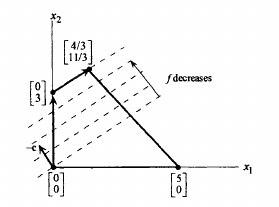
\includegraphics[scale=0.7]{ejemplo}
	\caption{Dibujo del ejemplo}
\end{figure}
\end{example}

\section{Algoritmo del Símplex}
\begin{itemize}
\item Inicialización: encontrar un punto extremo $\overline{x}$ con base $B$.
\item Iteraciones: Calcular $c'_N-c'_B B^{-1}N\equiv c'_N-z_N\equiv \overline{c}_N$. Si este vector es no negativo, paramos(la solución $\overline{x}$ es óptima). En caso contrario, $\exists j\mid c_j-c_B B^{-1}a_j<0$ (si hubiera más de un negativo, elegir el de mayor valor absoluto). Si $y_j=B^{-1}a_j\leq 0$ el problema no tiene mínimo (el mínimo sería $-\infty$). Si $y_{ij}\not\leq 0$ comenzar nuevamente las iteraciones tomando como punto extremo en la inicialización $\hat{x}=\overline{x}+\frac{\overline{b}_r}{y_{rj}}d_j$, siendo $\frac{\overline{b_r}}{y_{rj}}=\min\{\frac{\overline{b_i}}{y_{ij}}:y_{ij}>0\}$, $\overline{b}=B^{-1}b$, $y_j=B^{-1}a_j$, $d_j=\begin{pmatrix}
-y_j\\
e_j
\end{pmatrix}$,
siendo la nueva base la resultante de eliminar la columna $a_r$ de $B$ y en su lugar introducir la columna $a_j$.
\end{itemize}
Este algoritmo tiene el problema de determinar el extremo inicial. Para ello usamos el siguiente método.
\subsection{Método de M-grande}
Consiste en utilizar un problema auxiliar $(P_m)$.
\begin{align*}
 \min\ & c'x+M1^t x_h\qquad \equiv &\min c'x+M\sum_{i=1}^m x_{h_i}\\
&sa:\ Ax+Ix_h=b              & A_1x+ x_{h_1}=b_1 \\
& x\geq 0, x_h\in R^m_+    & \vdots \\
&                          & A_m+ x_{h_m}=b_m
\end{align*}
Donde $A_i$ representa la fila $i$ de la matriz $A$ y $M$ es una constante lo bastante grande (podemos considerar $M=\infty$).  En $P_m$ hay una base obvia $B=[\text{columnas de }x_h]=I$ y $B^{-1}=I\Rightarrow B^{-1}b\geq 0$ si $b\geq 0$. Esto permite aplicar el algoritmo del simplex a $P_m$ para hallar su solución óptima $x^*$. 

Si en $x^*$ hay alguna variable $x^*_{h_i}\neq 0$ para algún $i$, en el objetivo aparece $Mx^*_{h_i}$. Tenemos que $c'x<c'x^*$ para cualquier $x\in P$ (poliedro original), por lo que $P=\emptyset$, porque de haberlo el algoritmo habría encontrado uno más pequeño.  Si $x^*$ es tal que $x^*_h=0$, entonces $x^*$ es solución del problema original $(PL)$. 

\subsection{Forma tabular del algoritmo del símplex}

\begin{align*}
\min & c'x [B N]\\
& Ax=b\\
&x\geq 0
\end{align*}
\begin{tabular}{|c|c| c| c|c|}
\hline
 & & $c'_B$ & $c'_N$ & \\
 \hline
 $x_B$ & $c_B$ & $B$ & $N$ & $b$\\
 \hline

\end{tabular}$\underset{B^{-1},\overline{b}B^{-1}b\geq 0}{\Longrightarrow}$
\begin{tabular}{|c|c| c| c|c|}
\hline
 & & $c'_B$ & $c'_N$ & \\
 \hline
 $x_B$ & $B^{-1}B=I$ & $B^{-1}N=Y$ & $N$ & $\overline{b}$\\
 \hline

\end{tabular}

Apliquemos esto al ejemplo anterior.
\begin{align*}
\min &x_1-3x_2\\
sa & -x_1+2x_2+x_3 \quad = 6\\
   & x_1+x_2 \qquad +x_4 = 5\\
   &x_1,x_2,x_3,x_4\geq 0
\end{align*}
\begin{tabular}{|c|c| c c| c c|c|}

&             &     $c'_N$ & & $c'_B$ & & \\
\hline
 &            & $1$ & $-3$ & $0$ & $0$ & $b$  \\
 \hline
 $x_3$ & $0$ & $-1$ & $2$ &   $1$ &   $0$ & $6$\\
  $x_4$ & $0$ & $1$ & $1$ &    $0$ &  $1$ & $5$\\
 \hline
 &            & $1$ & $\boxed{-3}$ & $0$ & $0$ & Aquí se puede poner $-c_BB^{-1}b$ (objetivo)\\
 \hline
 &             &  $c_N -c_BB^{-1}N$ & & vector $0$& &

\end{tabular}

Hemos señalado el elemento no positivo. \\

Llamamos $N$ y $B$ respectivamente a las matrices cuadradas que se observan.  Llamamos además $y_i$ a los vectores columna ($y_0$ representa los valores de las variables y $y_1$ es la primera columna de $B$). Para conseguir el vector bajo $B$ hacemos $c_B-v_1 B$. Análogamente, para el otro vector hacemos $c_N-v_2 N$. Tenemos que el elemento negativo (en caso de haber más de uno, el más negativo) está bajo $y_2$, que es la segunda columna de la matriz $B$. A partir de eso calculamos $\min\{\frac{6}{2}, \frac{5}{1}\}=3$, es decir, calculamos el mínimo de los $\frac{b_i}{y_i}$ con $i\geq 1$ siempre que $y_i>0$. Este mínimo corresponde a la primera fila de $B$, esto es, a la variable $x_3$. Recordemos que las filas de se asocian a las variables básicas escritas a la izquierda y que las columnas se asocian a las variables colocadas en orden (esto es $y_i\rightarrow x_i$). Ahora nos interesa que la columna $\begin{vmatrix}
1\\
0
\end{vmatrix}$ aparezca en el lugar de la columna $\begin{vmatrix}
2\\
1
\end{vmatrix}$, puesto que $x_2$ se ha convertido por lo anterior en variable básica sustituyendo a $x_3$, y las variables básicas conforman una matriz identidad. Para ello, debemos realizar operaciones por filas. En este caso, basta hacer $\frac{1}{2}F_1$ y a continuación $F_2-F_1$, resultando la tabla siguiente

\begin{tabular}{|c|c| c c| c c|c|}
\hline
 &            & $1$ & $-3$ & $0$ & $0$ & $b$  \\
 \hline
 $x_2$ & $-3$ & $-\frac{1}{2}$ & $1$ &   $\frac{1}{2}$ &   $0$ & $3$\\
  $x_4$ & $0$ & $\frac{3}{2}$ & $0$ &    $-\frac{1}{2}$ &  $1$ & $2$\\
 \hline
 &            & $\boxed{-\frac{1}{2}}$ & $0$ & $\frac{3}{2}$ & $0$ & \\
 \hline

\end{tabular}\

Ahora operamos igual que antes tenemos que el mínimo es $\frac{4}{3}$, y deberíamos seguir así sucesivamente hasta que no quede ningún elemento en la fila inferior que sea negativo.

\end{document}